%! TeX program = lualatex
\documentclass[12pt,a4paper]{article}

\usepackage[nil]{babel}
\usepackage{unicode-math}
\usepackage[svgnames]{xcolor}
\usepackage{lmodern}
\usepackage{graphicx}
\usepackage{wrapfig}
\usepackage{float}
\usepackage{parskip}
\usepackage{enumitem}

\makeatother
\babelprovide[import=el, main, onchar=ids fonts]{greek} % can also do import=el-polyton
\babelprovide[import, onchar=ids fonts]{english}

\babelfont{rm}
          [Language=Default]{Liberation Sans}
\babelfont[english]{rm}
          [Language=Default]{Liberation Sans}
\babelfont{sf}
          [Language=Default]{Liberation Sans}
\babelfont{tt}
          [Language=Default]{Liberation Sans}

%Enter Title Here
\title{Use-cases-v1.0 \\ LibShare}
\author{\textbf{Ονόματα / ΑΜ / Έτος:} \\ Γρηγόρης Καπαδούκας / 1072484 / 4\textdegree \\ Χρήστος Μπεστητζάνος / 1072615 / 4\textdegree \\ Νικόλαος Αυγέρης / 1067508 / 5\textdegree \\ Περικλής Κοροντζής / 1072563 / 4\textdegree}

\begin{document}

\makeatletter
\begin{center}
	\LARGE{\@title} \\
	\pagebreak
	\begin{LARGE}\@author\end{LARGE} \\
\end{center}
\pagebreak

%Insert Body Here
\section{Use Case Diagram}

Το Use Case Diagram που φτιάξαμε αποτελεί το Σχήμα \ref{Use Case Diagram}. Για την καλύτερη και πιο λεπτομερή σχεδίαση, πολλά use cases τα οποία αποτελούν ένα use case παρακάτω στο κεφάλαιο \ref{Ροές των Use Cases}, εδώ έχουν αποτελέσει περισσότερα από ένα με σκοπό την καλύτερη ανάλυση της αλληλεπίδρασης μεταξύ των use cases.

Έτσι για παράδειγμα, το use case της "Αναζήτησης βιβλίων / χρήστη / αιτήσεων" στο κεφάλαιο \ref{Ροές των Use Cases} εδώ χωρίζεται σε "Αναζήτηση", "Αναζήτηση βιβλίου", "Αναζήτηση χρήστη" και "Αναζήτηση αίτησης", με σχέση γενίκευσης των τριών τελευταίων από το πρώτο. Επίσης τα use cases "Επεξεργασία Λίστας Αγαπημένων" και "Προβολή Ειδοποιήσεων" αποτελούν πάλι ένα use case στο κεφάλαιο \ref{Ροές των Use Cases}. Με αυτόν τον τρόπο προσπαθούμε να δημιουργήσουμε ένα αναλυτικό και κατανοητό use case diagram, αλλά και να αποφύγουνε να αναλύσουμε τετριμμένα use cases έπειτα.

Σημειώνω επίσης ότι όλοι οι χρήστες του συστήματος είναι ισάξιοι, και μπορούν να αποτελέσουν και Ενοικιαστές και Ιδιοκτήτες σε διαφορετικές συναλλαγές. Στο διάγραμμα έχουμε χρησιμοποιήσει τη σχέση γενίκευσης του Ενοικιαστή και του Ιδιοκτήτη με τον Χρήστη, ώστε να δηλώσουμε ότι τα use cases "Αποδοχή Προσφοράς Βιβλίου και Ενοικίαση" και "Αποδοχή Αίτησης Βιβλίου και Ενοικίαση" απαιτούν την συμμετοχή δύο χρηστών με διαφορετικούς ρόλους κάθε φορά. Αυτό δεν σημαίνει ότι ο Ενοικιαστής μιας συναλλαγής δεν γίνεται να είναι ο Ιδιοκτήτης της επόμενης που θα συμμετάσχει.

\begin{figure}[H]
	\makebox[\textwidth]{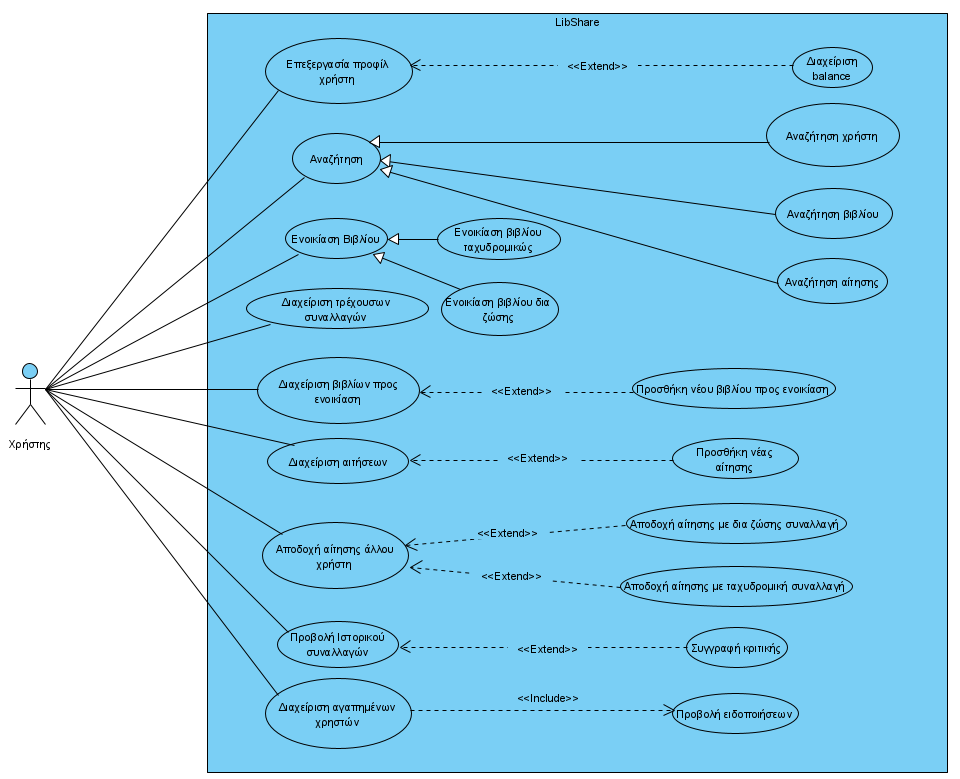
\includegraphics[width=\textwidth]{Use-case Diagram.png}}
	\caption{Use Case Diagram}
	\label{Use Case Diagram}
\end{figure}


\section{Ροές των Use Cases}
\label{Ροές των Use Cases}

\subsection{Αναζήτηση βιβλίων / χρήστη / αιτήσεων}

\subsubsection*{Βασική Ροή <<Αναζήτηση βιβλίων / χρήστη / αιτήσεων>>: Αναζήτηση βιβλίων με δια ζώσης συναλλαγή:}
\begin{enumerate}
    \item Ο χρήστης επιλέγει να μεταβεί στη σελίδα αναζήτησης.
    \item Το σύστημα εμφανίζει στον χρήστη τη σελίδα αναζήτησης.
    \item Ο χρήστης επιλέγει φίλτρο αναζήτησης "βιβλία" και εισάγει ένα κείμενο αναζήτησης (μπορεί να είναι και τίτλος βιβλίου και όνομα συγγραφέα).
        \label{Επιλογή τύπου αναζήτησης}
    \item Το σύστημα ελέγχει αν υπάρχουν διαθέσιμα βιβλία προς ενοικίαση που πληρούν το κείμενο αναζήτησης.
        \label{Ύπαρξη βιβλίου}
    \item Το σύστημα δείχνει τη λίστα με τα διαθέσιμα βιβλία στον χρήστη, περιέχοντας τους πλήρεις τίτλους, το όνομα συγγραφέα, τη κατηγορία που ανήκει, την έκδοση και τον εκδοτικό οίκο.
    \item Ο χρήστης επιλέγει ένα από τα βιβλία.
    \item Το σύστημα φορτώνει τη λίστα των ιδιοκτητών που προσφέρουν το βιβλίο που επιλέχθηκε και την προβάλλει στο χρήστη, εμφανίζοντας το όνομα των χρηστών που προσφέρουν το βιβλίο, το email τους, τη πόλη που μένουν, το score τους, το τύπο συναλλαγής που προσφέρουν (συνάντηση δια ζώσης ή ταχυδρομική συναλλαγή) και τη τιμή του βιβλίου ανά μέρα. 
    \item Το σύστημα δίνει τη δυνατότητα στο χρήστη να επιλέξει έναν ιδιοκτήτη από τη λίστα για να γίνει συναλλαγή μαζί του. Η χρήση αυτής της λειτουργίας αυτής αναλύεται στο use case "Αποδοχή Προσφοράς Βιβλίου και Ενοικίαση".
\end{enumerate}

\subsubsection*{Εναλλακτική Ροή 1: Αναζήτηση χρήστη - Αυτός υπάρχει:}
\begin{enumerate}
    \item[\ref{Επιλογή τύπου αναζήτησης}.α.1.] Ο χρήστης επιλέγει φίλτρο αναζήτησης "χρήστης" και εισάγει ένα κείμενο αναζήτησης (το username του χρήστη που αναζητεί).
    \item[\ref{Επιλογή τύπου αναζήτησης}.α.2.] Το σύστημα ελέγχει αν υπάρχει άλλος χρήστης με το όνομα που ζήτησε ο χρήστης και βλέπει ότι υπάρχει.
    \item[\ref{Επιλογή τύπου αναζήτησης}.α.3.] Το σύστημα φορτώνει τις αξιολογήσεις που έχουν γίνει για τον χρήστη που αναζητήθηκε από άλλους χρήστες, αν αυτές υπάρχουν.
    \item[\ref{Επιλογή τύπου αναζήτησης}.α.4.] Το σύστημα προβάλλει στον χρήστη το προφίλ του χρήστη που αναζήτησε, δηλαδή το username του, το email του, την ηλικία του, τη πόλη που μένει, το τηλέφωνό του, τη περιγραφή που όρισε για το προφίλ του, το rating του και τις αξιολογήσεις του.
    \item[\ref{Επιλογή τύπου αναζήτησης}.α.5.] Το σύστημα επίσης δίνει στο χρήστη τη δυνατότητα να προσθέσει τον χρήστη που αναζήτησε στη λίστα των αγαπημένων (η δυνατότητα αυτή χρησιμοποιείται στο use case "Επεξεργασία λίστας αγαπημένων και χρήση συστήματος ειδοποιήσεων").
\end{enumerate}

\subsubsection*{Εναλλακτική Ροή 2: Αναζήτηση χρήστη - Αυτός δεν υπάρχει:}
\begin{enumerate}
    \item[\ref{Επιλογή τύπου αναζήτησης}.β.1.] Ο χρήστης επιλέγει φίλτρο αναζήτησης "χρήστης" και εισάγει ένα κείμενο αναζήτησης (το username του χρήστη που αναζητεί).
    \item[\ref{Επιλογή τύπου αναζήτησης}.β.2.] Το σύστημα ελέγχει αν υπάρχει άλλος χρήστης με το όνομα που ζήτησε ο χρήστης και βλέπει ότι δεν υπάρχει.
    \item[\ref{Επιλογή τύπου αναζήτησης}.β.3.] Το σύστημα εμφανίζει στο χρήστη κενή σελίδα αναζήτησης.
\end{enumerate}

\subsubsection*{Εναλλακτική Ροή 3: Αναζήτηση αίτησης - Αυτή υπάρχει:}
\begin{enumerate}
    \item[\ref{Επιλογή τύπου αναζήτησης}.γ.1.] Ο χρήστης επιλέγει φίλτρο αναζήτησης "αιτήσεις" και εισάγει ένα κείμενο αναζήτησης (το όνομα του βιβλίου για το οποίο αναζητά αν υπάρχουν αιτήσεις ή το όνομα κάποιου συγγραφέα).
    \item[\ref{Επιλογή τύπου αναζήτησης}.γ.2.] Το σύστημα ελέγχει αν υπάρχει αίτηση που να πληρεί τα κριτήρια αναζήτησης που ζήτησε ο χρήστης και διαπιστώνει ότι υπάρχει.
    \item[\ref{Επιλογή τύπου αναζήτησης}.γ.3.] Το σύστημα δείχνει τη λίστα με τα βιβλία για τα οποία υπάρχουν αιτήσεις που πληρούν τα κριτήρια αναζήτησης στον χρήστη, περιέχοντας τους πλήρεις τίτλους, το όνομα συγγραφέα, τη κατηγορία που ανήκει, την έκδοση και τον εκδοτικό οίκο.
    \item[\ref{Επιλογή τύπου αναζήτησης}.γ.4.] Ο χρήστης επιλέγει ένα από τα βιβλία.
    \item[\ref{Επιλογή τύπου αναζήτησης}.γ.5.] Το σύστημα φορτώνει τη λίστα των χρηστών που έχουν κάνει αίτηση για το βιβλίο που επιλέχθηκε και την προβάλλει στον χρήστη, εμφανίζοντας το username των χρηστών που προσφέρουν το βιβλίο, το email τους, τη πόλη που μένουν, το score τους, το τύπο συναλλαγής που προσφέρουν (συνάντηση δια ζώσης ή ταχυδρομική συναλλαγή) και τη τιμή του βιβλίου ανά μέρα που προτίθενται να πληρώσουν.
    \item[\ref{Επιλογή τύπου αναζήτησης}.γ.6.] Το σύστημα δίνει τη δυνατότητα στο χρήστη να επιλέξει έναν χρήστη από τη λίστα για να εκπληρώσει την αίτησή του και να γίνει συναλλαγή μαζί του. Η χρήση αυτής της λειτουργίας αυτής αναλύεται στο use case "Αποδοχή Αίτησης Βιβλίου και Ενοικίαση".
\end{enumerate}

\subsubsection*{Εναλλακτική Ροή 4: Αναζήτηση αίτησης - Αυτή δεν υπάρχει:}
\begin{enumerate}
    \item[\ref{Επιλογή τύπου αναζήτησης}.δ.1.] Ο χρήστης επιλέγει φίλτρο αναζήτησης "αιτήσεις", και εισάγει ένα κείμενο αναζήτησης (το όνομα του βιβλίου για το οποίο αναζητά αν υπάρχουν αιτήσεις ή το όνομα ενός συγγραφέα).
    \item[\ref{Επιλογή τύπου αναζήτησης}.δ.2.] Το σύστημα ελέγχει αν υπάρχει αίτηση για το βιβλίο που αναζήτησε ο χρήστης και διαπιστώνει ότι δεν υπάρχει.
    \item[\ref{Επιλογή τύπου αναζήτησης}.δ.3.] Το σύστημα εμφανίζει στο χρήστη κενή σελίδα αναζήτησης.
\end{enumerate}

\subsubsection*{Εναλλακτική Ροή 5: Αναζήτηση βιβλίου - Αυτό δεν υπάρχει:}
\begin{enumerate}
    \item[\ref{Ύπαρξη βιβλίου}.1.] Το σύστημα ελέγχει αν υπάρχουν διαθέσιμα βιβλία προς ενοικίαση που να πληρούν το κείμενο αναζήτησης και βλέπει ότι δεν υπάρχουν.
    \item[\ref{Ύπαρξη βιβλίου}.2.] Το σύστημα εμφανίζει στο χρήστη κενή σελίδα αναζήτησης.
\end{enumerate}

\subsection{Αποδοχή Προσφοράς Βιβλίου και Ενοικίαση}
\label{Rental Use Case}
\subsubsection*{Βασική Ροή <<Αποδοχή Προσφοράς Βιβλίου και Ενοικίαση>>:}
\begin{enumerate}
    \item Ο ενοικιαστής κάνει προσφορά ενοικίασης στον ιδιοκτήτη που επέλεξε για το βιβλίο που αναζήτησε (στο use case της αναζήτησης).
        \label{Επιλογή τρόπου συναλλαγής}
    \item Το σύστημα επιβεβαιώνει ότι ο ενοικιαστής έχει αρκετά χρήματα στο λογαριασμό του για να καλύψει το "ποσό ασφαλείας" που θα δεσμευτεί αργότερα από τον λογαριασμό του.
        \label{Έλεγχος ποσού ασφαλείας}
    \item Το σύστημα δημιουργεί μια συναλλαγή σε κατάσταση αναμονής αποδοχής.
    \item Ο ιδιοκτήτης επιλέγει να προβάλλει τη σελίδα του Dashboard (όπου οι χρήστες βλέπουν τις τρέχουσες συναλλαγές τους).
    \item Το σύστημα μεταβιβάζει τον ιδιοκτήτη στη σελίδα του Dashboard.
    \item Ο ιδιοκτήτης αποδέχεται από τη σελίδα του Dashboard την προσφορά ενοικίασης.
    \item Το σύστημα επιβεβαιώνει ότι η προσφορά ενοικίασης έχει γίνει αποδεκτή από τον ιδιοκτήτη και αλλάζει την κατάσταση της συναλλαγής σε αποδεκτή.
        \label{Αποδοχή ή απόρριψη συναλλαγής}
    \item Το σύστημα δεσμεύει το ποσό ασφαλείας από το λογαριασμό του ενοικιαστή.
    \item Ο ενοικιαστής επιλέγει να προβάλλει τη σελίδα του Dashboard.
    \item Το σύστημα μεταβιβάζει τον ενοικιαστή στη σελίδα του Dashboard.
    \item Ο ενοικιαστής, αφού βρεθεί με τον ιδιοκτήτη δια ζώσης και παραλάβει το βιβλίο ή το βιβλίο φτάσει σε αυτόν μέσω ταχυδρομείου, ενημερώνει το σύστημα ότι έχει κατοχή του βιβλίου. 
    \item Ο ιδιοκτήτης επίσης ενημερώνει το σύστημα όταν έχει δώσει το βιβλίο ή όταν έχει φτάσει ταχυδρομικώς.
    \item Το σύστημα ελέγχει αν έλαβε ενημέρωση κατοχής του βιβλίου και από τον ενοικιαστή και από τον ιδιοκτήτη.
        \label {Δεν ενημερώνεται η κατοχή}
    \item Το σύστημα αρχίζει τη ημερήσια ανανέωση της συνολικής χρέωσης (προσθέτει το ημερήσιο χρέος κάθε μέρα στο συνολικό) και ελέγχει ημερησίως πάλι αν τα χρήματα του ενοικιαστή αρκούν για να καλύψουν τη χρέωση, και βλέπει ότι αυτό ισχύει κάθε φορά.
        \label{Τέλος χρημάτων}
    \item Ο ενοικιαστής, αφού τελειώσει το βιβλίο, βρίσκεται πάλι με τον ιδιοκτήτη και του δίνει το βιβλίο ή αποστέλλει πίσω το βιβλίο ταχυδρομικώς, και όταν αυτό βρίσκεται πλέον πίσω στην κατοχή του ιδιοκτήτη το σύστημα για την επιστροφή του βιβλίου.
    \item Ο ιδιοκτήτης επίσης ενημερώνει το σύστημα για την επιστροφή του βιβλίου όταν το παραλάβει.
        \label{Επιστροφή βιβλίου - Τέλος λεφτά δεν φτάνουν}
    \item Το σύστημα ελέγχει ότι έχει λάβει ενημέρωση επιστροφής βιβλίου και από τα δύο μέλη. 
    \item Το σύστημα σταματάει την ημερήσια ανανέωση του συνολικού χρέους και τον ημερήσιο έλεγχο, μεταφέρει στον ιδιοκτήτη το συνολικό ποσό του χρέους που προέκυψε και επιστρέφει το "ποσό ασφαλείας" στον ενοικιαστή. Επίσης μετατρέπει την κατάσταση της συναλλαγής σε ολοκληρωμένη.
        \label{Τέλος ενοικίασης}
\end{enumerate}

\subsubsection*{Εναλλακτική Ροή 1: Ο ενοικιαστής δεν έχει αρκετό υπόλοιπο για να καλύψει το "ποσό ασφαλείας":}
\begin{enumerate}
    \item[\ref{Έλεγχος ποσού ασφαλείας}.1.] Το σύστημα παρατηρεί ότι ο ενοικιαστής δεν έχει αρκετό χρηματικό ποσό στο λογαριασμό για να καλύψει το "ποσό ασφαλείας".
    \item[\ref{Έλεγχος ποσού ασφαλείας}.2.] Ο ενοικιαστής ενημερώνεται από το σύστημα ότι δεν έχει αρκετά χρήματα στον λογαριασμό του για να ξεκινήσει νέα συναλλαγή.
\end{enumerate}

\subsubsection*{Εναλλακτική Ροή 2: Η συναλλαγή απορρίπτεται από τον ιδιοκτήτη:}
\begin{enumerate}
    \item[\ref{Αποδοχή ή απόρριψη συναλλαγής}.1.] Το σύστημα παρατηρεί ότι η προσφορά ενοικίασης απορρίπτεται από τον ιδιοκτήτη, και αλλάζει τη κατάσταση της συναλλαγής που δημιουργήθηκε σε "Απορρίφθηκε".
    \item[\ref{Αποδοχή ή απόρριψη συναλλαγής}.2.] Η συναλλαγή ολοκληρώνεται και αποθηκεύεται (ως ακυρωμένη) στο ιστορικό συναλλαγών των δύο χρηστών από το σύστημα.
\end{enumerate}

\subsubsection*{Εναλλακτική Ροή 3: Τέλος χρημάτων ενοικιαστή}
\begin{enumerate}
    \item[\ref{Τέλος χρημάτων}.1.] Το σύστημα αρχίζει τη ημερήσια ανανέωση της συνολικής χρέωσης (προσθέτει το ημερήσιο χρέος κάθε μέρα στο συνολικό) και ελέγχει ημερησίως πάλι αν τα χρήματα του ενοικιαστή αρκούν για να καλύψουν τη χρέωση, και βλέπει ότι κάποτε δεν ισχύει.
    \item[\ref{Τέλος χρημάτων}.2.] Το σύστημα στέλνει το "ποσό ασφαλείας" στον ιδιοκτήτη.
    \item[\ref{Τέλος χρημάτων}.3.] Το σύστημα αλλάζει τη κατάσταση της συναλλαγής σε ολοκληρωμένη.
\end{enumerate}

\textbf{Σημείωση:} Σημειώνουμε εδώ ότι η "προσφορά ενοικίασης" υπάρχει ώστε ο ιδιοκτήτης να μπορεί να δει το "σκορ" του άλλου χρήστη και να αποφασίσει αν θέλει να κάνει συναλλαγή μαζί του ή όχι.

Επίσης ο λόγος που το σύστημα περιμένει και από τους δύο χρήστες την δήλωση αλλαγής κατοχής του βιβλίου και επιστροφής είναι για να προστατεύονται οι χρήστες και να μην προχωρήσει η συναλλαγή αν δεν υπάρχει συμφωνία.

Στη περίπτωση που ο ένας χρήστης κάνει δήλωση αλλαγής κατοχής ή επιστροφής και δεν το κάνει ο άλλος, το σύστημα δεν προχωρά τη συναλλαγή και θεωρούμε πως οι χρήστες θα χρησιμοποιήσουν το feature της επικοινωνίας με την εξυπηρέτηση πελατών για να λυθεί το θέμα.

Παρόλα αυτά τα use case της υποστήριξης των πελατών και της επίλυσης διαφωνιών χρηστών από τη μεριά της υποστήριξης πελατών έχουμε επιλέξει να μην τα αναλύσουμε για την συγκεκριμένη άσκηση.


\subsection{Αποδοχή Αίτησης Βιβλίου και Ενοικίαση}

\textbf{Σημείωση:} Αυτό το Use Case είναι κατά μεγάλο μέρος ίδιο με το "Αποδοχή Προσφοράς Βιβλίου και Ενοικίαση". Η κύρια διαφορά είναι ότι σε αυτό το use case, ο ιδιοκτήτης κάνει την "προσφορά εκπλήρωσης αίτησης" και ο ενοικιαστής την αποδέχεται, ενώ στο use case "Αποδοχή Προσφοράς Βιβλίου και Ενοικίαση" ο ενοικιαστής δημιουργεί "προσφορά ενοικίασης" και ο ιδιοκτήτης την αποδέχεται.

Σημειώνουμε εδώ ότι η "προσφορά εκπλήρωσης αίτησης" υπάρχει ώστε ο ενοικιαστής να μπορεί να δει το "σκορ" του άλλου χρήστη και να αποφασίσει αν θέλει να κάνει συναλλαγή μαζί του ή όχι.

Ο λόγος που παρουσιάζουμε το use case αυτό ξεχωριστό είναι επειδή δεν είχε αρκετά μεγάλη νοηματική συσχέτιση για να θεωρηθεί εναλλακτική ροή του "Αποδοχή Προσφοράς Βιβλίου και Ενοικίαση", αλλά ταυτόχρονα θέλαμε να το παρουσιάσουμε και να το υλοποιήσουμε για λόγους πληρότητας.

\subsubsection*{Βασική Ροή <<Αποδοχή Αίτησης Βιβλίου και Ενοικίαση>>:}
\begin{enumerate}
    \item Ο ιδιοκτήτης κάνει προσφορά εκπλήρωσης αίτησης στον ενοικιαστή που επέλεξε για το βιβλίο που αναζήτησε (στο use case της αναζήτησης).
    \item Το σύστημα επιβεβαιώνει ότι ο ενοικιαστής έχει αρκετά χρήματα στο λογαριασμό του για να καλύψει το "ποσό ασφαλείας" που θα δεσμευτεί αργότερα από τον λογαριασμό του.
    \item Το σύστημα δημιουργεί μια συναλλαγή σε κατάσταση αναμονής αποδοχής.
    \item Ο ενοικιαστής επιλέγει να προβάλλει τη σελίδα του Dashboard (όπου οι χρήστες βλέπουν τις τρέχουσες συναλλαγές τους).
    \item Το σύστημα μεταβιβάζει τον ενοικιαστή στη σελίδα του Dashboard.
    \item Ο ενοικιαστής αποδέχεται από τη σελίδα του Dashboard την προσφορά εκπλήρωσης αίτησης.
    \item Το σύστημα επιβεβαιώνει ότι η προσφορά εκπλήρωσης αίτησης έχει γίνει αποδεκτή από τον ενοικιαστή και αλλάζει την κατάσταση της συναλλαγής σε αποδεκτή.
    \item Το σύστημα δεσμεύει το ποσό ασφαλείας από το λογαριασμό του ενοικιαστή.
    \item Ο ιδιοκτήτης επιλέγει να προβάλλει τη σελίδα του Dashboard.
    \item Το σύστημα μεταβιβάζει τον ιδιοκτήτη στη σελίδα του Dashboard.
    \item Ο ενοικιαστής, αφού βρεθεί με τον ιδιοκτήτη δια ζώσης και παραλάβει το βιβλίο ή το βιβλίο φτάσει σε αυτόν μέσω ταχυδρομείου, ενημερώνει το σύστημα ότι έχει κατοχή του βιβλίου. 
    \item Ο ιδιοκτήτης επίσης ενημερώνει το σύστημα όταν έχει δώσει το βιβλίο ή όταν έχει φτάσει ταχυδρομικώς.
    \item Το σύστημα ελέγχει αν έλαβε ενημέρωση κατοχής του βιβλίου και από τον ενοικιαστή και από τον ιδιοκτήτη.
    \item Το σύστημα αρχίζει τη ημερήσια ανανέωση της συνολικής χρέωσης (προσθέτει το ημερήσιο χρέος κάθε μέρα στο συνολικό) και ελέγχει ημερησίως πάλι αν τα χρήματα του ενοικιαστή αρκούν για να καλύψουν τη χρέωση, και βλέπει ότι αυτό ισχύει κάθε φορά.
    \item Ο ενοικιαστής, αφού τελειώσει το βιβλίο, βρίσκεται πάλι με τον ιδιοκτήτη και του δίνει το βιβλίο ή αποστέλλει πίσω το βιβλίο ταχυδρομικώς, και όταν αυτό βρίσκεται πλέον πίσω στην κατοχή του ιδιοκτήτη το σύστημα για την επιστροφή του βιβλίου.
    \item Ο ιδιοκτήτης επίσης ενημερώνει το σύστημα για την επιστροφή του βιβλίου όταν το παραλάβει.
    \item Το σύστημα ελέγχει ότι έχει λάβει ενημέρωση επιστροφής βιβλίου και από τα δύο μέλη. 
    \item Το σύστημα σταματάει την ημερήσια ανανέωση του συνολικού χρέους και τον ημερήσιο έλεγχο, μεταφέρει στον ιδιοκτήτη το συνολικό ποσό του χρέους που προέκυψε και επιστρέφει το "ποσό ασφαλείας" στον ενοικιαστή. Επίσης μετατρέπει την κατάσταση της συναλλαγής σε ολοκληρωμένη.
\end{enumerate}

\subsubsection*{Εναλλακτική Ροή 1: Ο ενοικιαστής δεν έχει αρκετό υπόλοιπο για να καλύψει το "ποσό ασφαλείας":}
\begin{enumerate}
    \item[2.1.] Το σύστημα παρατηρεί ότι ο ενοικιαστής δεν έχει αρκετό χρηματικό ποσό στο λογαριασμό για να καλύψει το "ποσό ασφαλείας".
    \item[2.2.] Ο ιδιοκτήτης ενημερώνεται από το σύστημα ότι ο ενοικιαστής δεν έχει αρκετά χρήματα στον λογαριασμό του για να ξεκινήσει νέα συναλλαγή.
\end{enumerate}

\subsubsection*{Εναλλακτική Ροή 2: Η συναλλαγή απορρίπτεται από τον ενοικιαστή}
\begin{enumerate}
    \item[7.1.] Το σύστημα παρατηρεί ότι η προσφορά εκπλήρωσης αίτησης απορρίπτεται από τον ενοικιαστή, και αλλάζει τη κατάσταση της συναλλαγής που δημιουργήθηκε σε "Απορρίφθηκε".
    \item[7.2.] Η συναλλαγή ολοκληρώνεται και αποθηκεύεται (ως ακυρωμένη) στο ιστορικό συναλλαγών των δύο χρηστών από το σύστημα.
\end{enumerate}

\subsubsection*{Εναλλακτική Ροή 3: Τέλος χρημάτων ενοικιαστή}
\begin{enumerate}
    \item[11.1.] Το σύστημα αρχίζει τη ημερήσια ανανέωση της συνολικής χρέωσης (προσθέτει το ημερήσιο χρέος κάθε μέρα στο συνολικό) και ελέγχει ημερησίως πάλι αν τα χρήματα του ενοικιαστή αρκούν για να καλύψουν τη χρέωση, και βλέπει ότι κάποτε δεν ισχύει.
    \item[11.2.] Το σύστημα στέλνει το "ποσό ασφαλείας" στον ιδιοκτήτη.
    \item[11.3.] Το σύστημα αλλάζει τη κατάσταση της συναλλαγής σε ολοκληρωμένη.
\end{enumerate}

\subsection{Διαχείριση των βιβλίων που προσφέρει ο χρήστης προς ενοικίαση από άλλους}

\subsubsection*{Βασική ροή <<Διαχείριση των βιβλίων που προσφέρει ο χρήστης \\προς ενοικίαση από άλλους>>: Προσθήκη και ενοικίαση βιβλίου από άλλον χρήστη:}
\begin{enumerate}
    \item Ο χρήστης επιλέγει να προβάλλει τη λίστα των βιβλίων που προσφέρει για ενοικίαση.
    \item Το σύστημα φορτώνει τη λίστα των βιβλίων και την εμφανίζει στον χρήστη.
    \item Το σύστημα δίνει στον χρήστη την επιλογή να προσθέσει βιβλία προς ενοικίαση, να αφαιρέσει και να επεξεργαστεί τις προσφορές βιβλίων που προσφέρει ήδη.
    \item Ο χρήστης επιλέγει να προσθέσει ένα νέο βιβλίο προς ενοικίαση από τους υπόλοιπους χρήστες.
    \item Ο χρήστης συμπληρώνει τα στοιχεία του βιβλίου (τίτλος, συγγραφέας, εκδοτικός οίκος και χρονολογία τύπωσης, κατηγορίες στις οποίες ανήκει το βιβλίο, τρόπος παράδοσης, τιμή, ποσότητα ίδιων βιβλίων) και ολοκληρώνει την προσθήκη.
    \item Το σύστημα καταγράφει τα στοιχεία του βιβλίου και ολοκληρώνει την προσθήκη.
    \item Το σύστημα δημιουργεί ειδοποιήσεις για όλους τους χρήστες που έχουν τον χρήστη που πρόσθεσε τη προσφορά βιβλίου ως αγαπημένο.
    \item Το σύστημα φορτώνει ξανά τη σελίδα όπου φαίνεται η προσθήκη.
\end{enumerate}

\subsubsection*{Εναλλακτική ροή 1: Ο χρήστης δεν έχει εισάγει προηγουμένως βιβλία προς ενοικίαση από άλλους χρήστες:}
\begin{enumerate}
    \item [2.1.] Το σύστημα αντιλαμβάνεται ότι ο χρήστης δεν έχει προσθέσει προηγουμένως βιβλία προς ενοικίαση.
    \item [2.2.] Το σύστημα ενημερώνει αντίστοιχα τον χρήστη.
    \item [2.3.] Η ροή συνεχίζεται από το βήμα 3 της βασικής ροής.
\end{enumerate}

\subsubsection*{Εναλλακτική ροή 2: Ο χρήστης επιλέγει να επεξεργαστεί μια προσφορά βιβλίου που έχει ήδη προσθέσει:}
\begin{enumerate}
    \item [4.α.1.] Ο χρήστης επιλέγει να επεξεργαστεί μια προσφορά βιβλίου που έχει ήδη προσθέσει.
    \item [4.α.2.] Ο χρήστης συμπληρώνει τις πληροφορίες που θέλει να ανανεώσει για τη τιμή ανά μέρα και τον τύπο συναλλαγής (δια ζώσης συναλλαγή ή ταχυδρομική).
    \item [4.α.3.] Το σύστημα καταγράφει τις αλλαγές.
    \item [4.α.4.] Το σύστημα φορτώνει ξανά τη σελίδα όπου φαίνονται οι αλλαγές.
\end{enumerate}

\subsubsection*{Εναλλακτική ροή 3: Ο χρήστης επιλέγει να διαγράψει ένα από τα βιβλία από τη λίστα των βιβλίων που προσφέρει προς ενοικίαση:}
\begin{enumerate}
    \item [4.β.1.] Ο χρήστης επιλέγει να αλλάξει διαγράψει ένα βιβλίο από τη λίστα αυτών που προσφέρει.
    \item [4.β.2.] Το σύστημα διαγράφει το βιβλίο από τη λίστα των διαθέσιμων βιβλίων του χρήστη.
    \item [4.β.3.] Το σύστημα φορτώνει ξανά τη σελίδα όπου φαίνονται οι αλλαγές.
\end{enumerate}

\subsection{Διαχείριση των αιτήσεων που έχει κάνει ο χρήστης}

\subsubsection*{Βασική ροή <<Διαχείριση των αιτήσεων που έχει κάνει ο χρήστης>>: Προσθήκη νέου αιτήματος:}
\begin{enumerate}
    \item Ο χρήστης επιλέγει να δει τη λίστα με τα αιτήματά του. 
    \item Το σύστημα ψάχνει αν υπάρχουν αιτήματα και αν υπάρχουν εμφανίζει οθόνη με τα ήδη υπάρχοντα αιτήματά του μαζί με στοιχεία του καθενός από αυτά. 
    \item Ο χρήστης επιλέγει να προσθέσει καινούριο αίτημα.
    \item Ο χρήστης εισάγει τα στοιχεία του βιβλίου τα οποία θέλει να αποκτήσει, προσθέτοντας την τιμή που προτίθεται να πληρώσει. 
    \item Το σύστημα αναζητά αν αυτό το βιβλίο υπάρχει ήδη διαθέσιμο από κάποιον άλλο χρήστη που το προσφέρει ήδη στην πλατφόρμα. 
    \item Το σύστημα προχωράει στην καταχώρηση του αιτήματος. 
    \item Το σύστημα τον ενημερώνει για την επιτυχή καταχώρηση του αιτήματος. 
    \item Ο χρήστης κλείνει το αίτημα
    \item Εμφανίζεται η λίστα των αιτημάτων ανανεωμένη με το νέο αίτημα.
\end{enumerate}

\subsubsection*{Εναλλακτική ροή 1: Ο χρήστης δεν έχει κάνει προηγούμενες αιτήσεις:}
\begin{enumerate}
    \item[2.1.] Το σύστημα αντιλαμβάνεται ότι o χρήστης δεν έχει κάνει καμία προηγούμενη αίτηση, οπότε εμφανίζεται μια άδεια οθόνη με μοναδική λειτουργία την προσθήκη αίτησης.
    \item[2.2.] Η ροή συνεχίζεται από το βήμα 3 της βασικής ροής.
\end{enumerate}

\subsubsection*{Εναλλακτική ροή 2: Ο χρήστης αφαιρεί υπάρχουσα αίτηση:}
\begin{enumerate}
    \item[3.α.1] Ο χρήστης επιλέγει να διαγράψει μια αίτηση του.
    \item[3.α.2] Το σύστημα τον καλεί να επιβεβαιώσει την επιλογή του. 
    \item[3.α.3] Ο χρήστης επιβεβαιώνει.
    \item[3.α.4] Το σύστημα διαγράφει το request.
    \item[3.α.5] Εμφανίζεται πάλι η οθόνη των requests.
\end{enumerate}

\subsubsection*{Εναλλακτική ροή 3: Ο χρήστης κάνει edit υπάρχουσα αίτηση:}
\begin{enumerate}
    \item[3.β.1] Ο χρήστης επιλέγει να επεξεργαστεί κάποια υπάρχουσα αίτηση. 
    \item[3.β.2] Το σύστημα εμφανίζει μια καινούργια οθόνη με τα στοιχεία της αίτησης που επέλεξε. 
    \item[3.β.3] Ο χρήστης επιλέγει το στοιχείο που θέλει να αλλάξει και συμπληρώνει την καινούργια τιμή. 
    \item[3.β.4] Επιβεβαιώνει την επιλογή του.
    \item[3.β.5] Το σύστημα επιστρέφει το χρήστη στην οθόνη με τα στοιχεία. 
    \item[3.β.6] Ο χρήστης οριστικοποιεί.
    \item[3.β.7] Το σύστημα επιστρέφει την οθόνη με τα requests με τα ανανεωμένα στοιχεία.
\end{enumerate}

\subsubsection*{Εναλλακτική ροή 4: Το βιβλίο είναι ήδη διαθέσιμο προς ενοικίαση}
\begin{enumerate}
    \item[5.1] Το σύστημα βρίσκει ότι βιβλίο το οποίο ο χρήστης αναζητούσε υπάρχει ήδη διαθέσιμο προς ενοικίαση από άλλον χρήστη και 
    \item[5.2] Το σύστημα εμφανίζει στον χρήστη την υπάρχουσα προσφορά με τα στοιχεία της και δυνατότητα ενοικίασης του, αν αυτός επιθυμεί.
\end{enumerate}

\subsection{Αξιολόγηση άλλων χρηστών μετά από την ολοκλήρωση συναλλαγής}

\subsubsection*{Βασική ροή <<Αξιολόγηση άλλων χρηστών μετά από την ολοκλήρωση συναλλαγής>>: Προσθήκη νέας αξιολόγησης με το προαιρετικό σχόλιο}
\begin{enumerate}
    \item Από την οθόνη του ιστορικού συναλλαγών ο χρήστης επιλέγει μια συναλλαγή και διαλέγει να αξιολογήσει τον χρήστη με τον οποίο έκανε τη συναλλαγή. 
    \item Το σύστημα εμφανίζει μια επιλογή για αξιολόγηση της μορφής 1-5 αστεριών, μαζί με προαιρετική προσθήκη σχολίου. 
    \item Ο χρήστης επιλέγει να κάνει αξιολόγηση μόνο με βάση τα αστεράκια. 
    \item Το σύστημα εμφανίζει την επιλογή αξιολόγησης 1-5 (αστέρια). 
    \item Ο χρήστης κάνει την επιλογή του και επιβεβαιώνει.
    \item Το σύστημα αποθηκεύει την αξιολόγηση και ενημερώνει τον χρήστη για την επιτυχία της ενέργειάς του.
    \item Το σύστημα επιστρέφει τον χρήστη στην οθόνη του ιστορικού.
\end{enumerate}

\subsubsection*{Εναλλακτική ροή 1: Ο χρήστης κάνει αξιολόγηση χωρίς το προαιρετικό σχόλιο}
\begin{enumerate}
    \item[3.1] Ο χρήστης επιλέγει γραπτή αξιολόγηση μαζί με το προαιρετικό σχόλιο. 
    \item[3.2] Το σύστημα εμφανίζει επιλογή αξιολόγησης 1-5 (αστέρια), μαζί με ένα text field για το σχόλιο. 
    \item[3.3] Ο χρήστης συμπληρώνει το σχόλιο και τα αστεράκια και επιβεβαιώνει
    \item[3.4] Επιστροφή στο βήμα 6 της βασικής ροής.
\end{enumerate}

\subsection{Προβολή και Επεξεργασία στοιχείων λογαριασμού χρήστη}

\subsubsection*{Βασική ροή <<Προβολής και επεξεργασίας στοιχείων λογαριασμού \\χρήστη>>:}
\begin{enumerate}
    \item Ο χρήστης επιλέγει να πάει στη σελίδα του προφίλ. 
    \item Το σύστημα φορτώνει τα στοιχεία του χρήστη (username, email, περιγραφή, τοποθεσία και τηλέφωνο) και τα εμφανίζει στον χρήστη.
    \item Ο χρήστης επιλέγει να κάνει επεξεργασία των στοιχείων του και εισάγει νέα στοιχεία για αυτά που θέλει να αλλάξει (εκτός του password και της εικόνας χρήστη που αναλύονται σε εναλλακτική ροή και του email που δεν μπορεί να αλλάξει). 
    \item Το σύστημα ελέγχει αν τα στοιχεία έχουν τη σωστή μορφοποίηση, δηλαδή το username να έχει εύρος από 1-20 χαρακτήρες και δεν το έχει ήδη άλλος χρήστης, η περιγραφή να είναι από 1 με 150 χαρακτήρες, η τοποθεσία να είναι από 1 έως 35 χαρακτήρες και το κινητό να είναι δεκαψήφιος αριθμός και βλέπει ότι οι κανόνες τηρούνται.
    \item Το σύστημα καταγράφει τις αλλαγές.
    \item Το σύστημα επιστρέφει τον χρήστη στην οθόνη του προφίλ του, όπου μπορεί να δει το ανανεωμένο προφίλ του.
\end{enumerate}

\subsubsection*{Εναλλακτική ροή 1: Ο χρήστης επιθυμεί αλλαγή του κωδικού:}
\begin{enumerate}
    \item [3.α.1.] Ο χρήστης επιλέγει αλλαγή του κωδικού του. 
    \item [3.α.2.] Το σύστημα του ζητάει να συμπληρώσει τον παλιό κωδικό του και τον νέο κωδικό που θέλει δύο φορές (η δεύτερη για επαλήθευση).
    \item [3.α.3.] Ο χρήστης συμπληρώνει τον παλιό κωδικό και τον νέο κωδικό του δύο φορές.
    \item [3.α.4.] Το σύστημα ελέγχει αν ο παλιός κωδικός είναι σωστός και ότι οι δύο νέοι κωδικοί είναι ίδιο και βλέπει ότι αυτό ισχύει.
    \item [3.α.5.] Το σύστημα ανανεώνει τον κωδικό πρόσβασης του χρήστη.
\end{enumerate}

\subsubsection*{Εναλλακτική ροή 2: Ο παλιός κωδικός κατά την αλλαγή κωδικού δεν είναι σωστός ή οι δύο νέοι κωδικοί δεν είναι ίδιοι:}
\begin{enumerate}
    \item [3.β.1.] Ο χρήστης επιλέγει αλλαγή του κωδικού του.
    \item [3.β.2.] Το σύστημα του ζητάει να συμπληρώσει τον παλιό κωδικό του και τον νέο κωδικό που θέλει δύο φορές (η δεύτερη για επαλήθευση).
    \item [3.β.3.] Ο χρήστης συμπληρώνει τον παλιό κωδικό και τον νέο κωδικό του δύο φορές.
    \item [3.β.4.] Το σύστημα ελέγχει αν ο παλιός κωδικός είναι σωστός και ότι οι δύο νέοι κωδικοί είναι ίδιο και βλέπει ότι αυτό δεν ισχύει.
    \item [3.β.5.] Το σύστημα εμφανίζει μήνυμα σφάλματος στο χρήστη.  
\end{enumerate}

\subsubsection*{Εναλλακτική ροή 3: Τα νέα στοιχεία που εισάγει ο χρήστης δεν τηρούν τους κανόνες μορφοποίησης:}
\begin{enumerate}
    \item [4.α.1.] Το σύστημα ελέγχει τα νέα στοιχεία (username, περιγραφή, τοποθεσία, τηλέφωνο) και δεν τηρούνται οι προδιαγραφές.
    \item [4.α.2.] Το σύστημα εμφανίζει μήνυμα σφάλματος στο χρήστη.
\end{enumerate}

\subsubsection*{Εναλλακτική ροή 4: Το νέο username χρησιμοποιείται ήδη από άλλον χρήστη:}
\begin{enumerate}
    \item [4.β.1.] Το σύστημα ελέγχει το νέο username και βλέπει ότι υπάρχει ήδη χρήστης με το username αυτό. 
    \item [4.β.2.] Το σύστημα εμφανίζει μήνυμα σφάλματος στο χρήστη.  
\end{enumerate}

\subsection{Επεξεργασία χρηματικού υπολοίπου χρήστη}

\textbf{Σημείωση:} Στο παρακάτω use case, επειδή δεν μπορούμε να δημιουργήσουμε πραγματικό σύστημα πληρωμών για την εργασία, με πραγματικό payment processor, αποφασίσαμε να σχεδιάζουμε για τη συγκεκριμένη άσκηση ένα σύστημα όπου ο χρήστης επιλέγει αυθαίρετα το ποσό που θέλει να προσθέσει ή να αφαιρέσει, και το σύστημα θα ελέγχει απλά αν το ποσό είναι έγκυρο (πχ έχει αρκετά χρήματα στο λογαριασμό ο χρήστης για να αφαιρέσει) και θα καταγράφει την αλλαγή στο χρηματικό υπόλοιπο.


\subsubsection*{Βασική ροή <<Επεξεργασίας χρηματικού υπολοίπου χρήστη>>: Προσθήκη χρημάτων:}
\begin{enumerate}
    \item Ο χρήστης επιλέγει να δει το χρηματικό του υπόλοιπο πηγαίνοντας στη σελίδα προφίλ.
    \item Το σύστημα εμφανίζει στον χρήστη το προφίλ του μαζί με το χρηματικό υπόλοιπό του και επιλογή επεξεργασίας του.
    \item Ο χρήστης επιλέγει να επεξεργαστεί το χρηματικό υπόλοιπό του.
    \item Το σύστημα εμφανίζει 2 επιλογές στο χρήστη, προσθήκη ή αφαίρεση χρημάτων, ώστε να συμπληρώσει όποια θέλει.
    \item Ο χρήστης επιλέγει προσθήκη χρημάτων, συμπληρώνοντας το αντίστοιχο ποσό που θέλει να προσθέσει.
    \item Το σύστημα ελέγχει αν η μορφοποίηση της εισόδου του χρήστη είναι έγκυρη (ποσό μεγαλύτερο του 0), το οποίο ισχύει.
    \item Το σύστημα προσθέτει τα λεφτά στο χρηματικό υπόλοιπο του χρήστη και τον επιστρέφει στη σελίδα προφίλ.
    \item Το νέο υπόλοιπο φαίνεται πλέον στην σελίδα του προφίλ του χρήστη.
\end{enumerate}

\subsubsection*{Εναλλακτική ροή 1: Επιλογή αφαίρεσης χρημάτων από τον λογαριασμό - Έγκυρο ποσό:}
\begin{enumerate}
    \item [5.α.1.] Ο χρήστης επιλέγει αφαίρεση χρημάτων, συμπληρώνοντας το αντίστοιχο ποσό που θέλει να αφαιρέσει.
    \item [5.α.2.] Το σύστημα ελέγχει αν η μορφοποίηση της εισόδου του χρήστη είναι έγκυρη (ποσό μεγαλύτερο του 0) καθώς και ότι υπάρχει αρκετά μεγάλο υπόλοιπο στο λογαριασμό για να γίνει η αφαίρεση, το οποίο ισχύει.
    \item [5.α.3.] Το σύστημα αφαιρεί τα λεφτά στο χρηματικό υπόλοιπο του χρήστη και τον επιστρέφει στη σελίδα προφίλ.
    \item [5.α.4.] Το νέο υπόλοιπο φαίνεται πλέον στην σελίδα του προφίλ του χρήστη.
\end{enumerate}

\subsubsection*{Εναλλακτική ροή 2: Επιλογή αφαίρεσης χρημάτων από τον λογαριασμό - Μη έγκυρο ποσό:}
\begin{enumerate}
    \item [5.β.1.] Ο χρήστης επιλέγει αφαίρεση χρημάτων, συμπληρώνοντας το αντίστοιχο ποσό που θέλει να αφαιρέσει.
    \item [5.β.2.] Το σύστημα ελέγχει αν η μορφοποίηση της εισόδου του χρήστη είναι έγκυρη (ποσό μεγαλύτερο του 0) καθώς και ότι υπάρχει αρκετά μεγάλο υπόλοιπο στο λογαριασμό για να γίνει η αφαίρεση, το οποίο δεν ισχύει.
    \item [5.β.3.] Το σύστημα εμφανίζει μήνυμα σφάλματος.
\end{enumerate}

\subsubsection*{Εναλλακτική ροή 3: Η μορφοποίηση της εισόδου του χρήστη είναι μη έγκυρη:}
\begin{enumerate}
    \item [6.1.] Το σύστημα ελέγχει αν η μορφοποίηση της εισόδου του χρήστη είναι έγκυρη (ποσό μεγαλύτερο του 0), το οποίο δεν ισχύει.
    \item [6.2.] Το σύστημα εμφανίζει μήνυμα σφάλματος.
\end{enumerate}

\subsection{Επεξεργασία λίστας αγαπημένων και χρήση \\συστήματος ειδοποιήσεων}

\subsubsection*{Βασική ροή <<Επεξεργασία λίστας αγαπημένων και χρήση συστήματος ειδοποιήσεων>>: Προσθήκη στην λίστα αγαπημένων και προβολή ειδοποίησης:}
\begin{enumerate}
    \item Ο χρήστης προβάλλει το προφίλ ενός χρήστη (από την αναζήτηση χρήστη) και επιλέγει να τον προσθέσει στη λίστα των αγαπημένων του.
    \item Το σύστημα ελέγχει αν υπάρχει ήδη προσθεμένος ο χρήστης στην λίστα αγαπημένων και βλέπει ότι αυτό δεν ισχύει.
    \item To σύστημα προσθέτει τον χρήστη που επιλέχθηκε στη λίστα αγαπημένων του αρχικού χρήστη.
    \item Ο χρήστης που προστέθηκε στη λίστα αγαπημένων προσθέτει ένα βιβλίο στην πλατφόρμα προς ενοικίαση ή κάνει μια νέα αίτηση (μέσω άλλων use cases, αναφέρουμε αυτό το βήμα και το επόμενο μόνο για λόγους πιο εύκολης κατανόησης της αλληλουχίας ενεργειών).
    \item Η πλατφόρμα το αντιλαμβάνεται και προσθέτει μια νέα ειδοποίηση στην οθόνη ειδοποιήσεων του αρχικού χρήστη. (Μέσω των ίδιων άλλων use cases)
    \item Ο αρχικός χρήστης επιλέγει να προβάλλει τις ειδοποιήσεις.
    \item Το σύστημα μεταφέρει τον χρήστη στη σελίδα ειδοποιήσεών του.
    \item Ο χρήστης βλέπει τη νέα ειδοποίηση που προστέθηκε και αποφασίζει να την αφαιρέσει από τη λίστα ειδοποιήσεών του.
    \item Το σύστημα αφαιρεί την ειδοποίηση από τη λίστα ειδοποιήσεων του χρήστη.
    \item Το σύστημα εμφανίζει ανανεωμένη τη λίστα ειδοποιήσεων στο χρήστη.
\end{enumerate}

\subsubsection*{Εναλλακτική ροή 1: Ήδη προσθεμένος χρήστης:}
\begin{enumerate}
    \item [2.1.] Το σύστημα ελέγχει αν υπάρχει ήδη προσθεμένος ο χρήστης στην λίστα αγαπημένων και βλέπει ότι αυτό ισχύει.
    \item [3.2.] Η ροή συνεχίζει από το βήμα 4 της βασικής ροής.
\end{enumerate}

\subsubsection*{Εναλλακτική ροή 2: Διαγραφή χρήστη από τη λίστα αγαπημένων:}
\begin{enumerate}
    \item [4.1.] Ο αρχικός χρήστης επιλέγει να δει την λίστα αγαπημένων του.
    \item [4.2.] Το σύστημα μεταφέρει τον χρήστη στη σελίδα αγαπημένων του.
    \item [4.3.] Ο χρήστης επιλέγει να αφαιρέσει ένα χρήστη από τη λίστα των αγαπημένων του.
    \item [4.2.] Το σύστημα αφαιρεί τον χρήστη αυτόν από τη λίστα αγαπημένων του αρχικού χρήστη.
    \item [4.3.] Το σύστημα εμφανίζει ανανεωμένη τη λίστα αγαπημένων στον αρχικό χρήστη.
\end{enumerate}

\subsection{Προβολή ιστορικού συναλλαγών και στατιστικών}

\subsubsection*{Βασική ροή <<Προβολή ιστορικού συναλλαγών και στατιστικών>>:}
\begin{enumerate}
    \item Ο χρήστης επιλέγει να προβάλλει το ιστορικό των συναλλαγών του μαζί με σχετικά στατιστικά.
    \item Το σύστημα αναζητεί και βρίσκει τις ολοκληρωμένες συναλλαγές που έχει κάνει ο χρήστης.
    \item Το σύστημα δείχνει στον χρήστη την λίστα των συναλλαγών.
    \item Το σύστημα επίσης επεξεργάζεται τα δεδομένα και δείχνει ένα bar chart σχετικά με το πλήθος των συναλλαγών του χρήστη ανά κατηγορία βιβλίου (fantasy, non-fiction κ.α.), όταν ο χρήστης είναι ο ιδιοκτήτης του βιβλίου.
    \item Το σύστημα επίσης επεξεργάζεται τα δεδομένα και δείχνει ένα bar chart σχετικά με το πλήθος των συναλλαγών του χρήστη ανά ηλικιακή ομάδα του ενοικιαστή (<21, 21 - 31, 32 - 41, 42 - 50, >50), όταν ο χρήστης είναι ο ιδιοκτήτης του βιβλίου.
    \item Το σύστημα ελέγχει για ποιες συναλλαγές ο χρήστης έχει κάνει αξιολόγηση του άλλου χρήστη.
    \item Το σύστημα δίνει τη δυνατότητα στο χρήστη για αξιολόγησης των χρηστών με τους οποίους ο χρήστης έχει κάνει συναλλαγή και δεν έχει κάνει αξιολόγηση για τη συναλλαγή αυτή. Αν ο χρήστης επιλέγει αυτή τη επιλογή μεταβιβάζεται στο use case "Αξιολόγηση άλλων χρηστών μετά από την ολοκλήρωση συναλλαγής".
\end{enumerate}

\subsubsection*{Εναλλακτική ροή 1: Το σύστημα δεν βρίσκει εγγραφές στο ιστορικό συναλλαγών:}
\begin{enumerate}
    \item [2.1.] Το σύστημα αντιλαμβάνεται ότι δεν έχει καταγράψει ολοκληρωμένες συναλλαγές για τον χρήστη.
    \item [2.2.] Το σύστημα εμφανίζει κενή σελίδα ιστορικού συναλλαγών.
\end{enumerate}

\section{Συμμετοχή και Ρόλοι στη Συγγραφή του Κειμένου}
\begin{enumerate}
	\item \textbf{Γρηγόρης Καπαδούκας:} Author (Κεφαλαίων 1, 2.1, 2.2, 2.3), Editor Όλων, Reviewer Όλων
	\item \textbf{Χρήστος Μπεστητζάνος:} Author (Κεφαλαίων 2.5, 2.6)
   	\item \textbf{Νικόλαος Αυγέρης:} Author (Κεφαλαίων 2.7, 2.8, 2.9)
	\item \textbf{Περικλής Κοροντζής:} Author (Κεφαλαίων 2.4, 2.10)
\end{enumerate}
\section{Αλλαγές από έκδοση σε έκδοση}

\subsection{Από έκδοση v0.1 σε έκδοση v0.2}
\begin{itemize}
    \item Διόρθωση του Use-Case Diagram
    \item Αλλαγή στο Use Case "Αναζήτηση βιβλίων / χρήστη / αιτήσεων"
    \item Αλλαγή στο Use Case "Ενοικίαση βιβλίου από άλλο χρήστη"
    \item Προσθήκη του Use Case "Ενοικίαση βιβλίου σε άλλο χρήστη (μεριά ιδιοκτήτη)"
    \item Αλλαγή στο Use Case "Διαχείριση των βιβλίων που προσφέρει ο χρήστης προς ενοικίαση από άλλους"
    \item Αλλαγή στο Use Case "Διαχείριση των αιτήσεων που κάνει ο χρήστης"
    \item Διαγραφή του use case "Εκπλήρωση αιτήσεων που έχουν κάνει άλλοι χρήστες"
    \item Αλλαγή στο Use Case "Αξιολόγηση άλλων χρηστών μετά από την ολοκλήρωση συναλλαγής"
    \item Αλλαγή στο Use Case "Προβολή και επεξεργασία στοιχείων λογαριασμού χρήστη"
    \item Αλλαγή στο Use Case "Επεξεργασία χρηματικού υπολοίπου χρήστη"
    \item Αλλαγή στο Use Case "Προβολή ιστορικού συναλλαγών και στατιστικών"
\end{itemize}
Άρα από την προηγούμενη έκδοση έχουν αλλάξει όλα τα Use-Cases εκτός του "Επεξεργασία λίστας αγαπημένων και χρήση συστήματος ειδοποιήσεων".

Σε ορισμένα από τα Use Cases οι αλλαγές είναι μεγάλες, σε άλλες η ουσία παραμένει ίδια με καλύτερο όμως διαχωρισμό των βημάτων και με μικρές διορθώσεις σε ορισμένα βήματα.

\subsection{Από έκδοση v0.2 σε έκδοση v0.3}
\begin{itemize}
    \item Αλλαγή στο Use Case "Αναζήτηση βιβλίων / χρήστη / αιτήσεων"
    \item Διαγραφή των Use Cases "Ενοικίαση βιβλίου από άλλο χρήστη" και "Ενοικίαση βιβλίου σε άλλο χρήστη (μεριά ιδιοκτήτη)" και αντικατάστασή τους με τα "Αποδοχή Προσφοράς Βιβλίου και Ενοικίαση" και "Αποδοχή Αίτησης Βιβλίου και Ενοικίαση".
    \item Προσθήκη της σημείωσης στο Use Case "Επεξεργασία χρηματικού υπολοίπου χρήστη".
\end{itemize}

\subsection{Από έκδοση v0.3 σε έκδοση v1.0}
\begin{itemize}
    \item Διόρθωση του use case Diagram
    \item Διορθώσεις στα use cases των κεφαλαίων 2.1, 2.2, 2.3
\end{itemize}

\end{document}
